\begin{figure}[t]
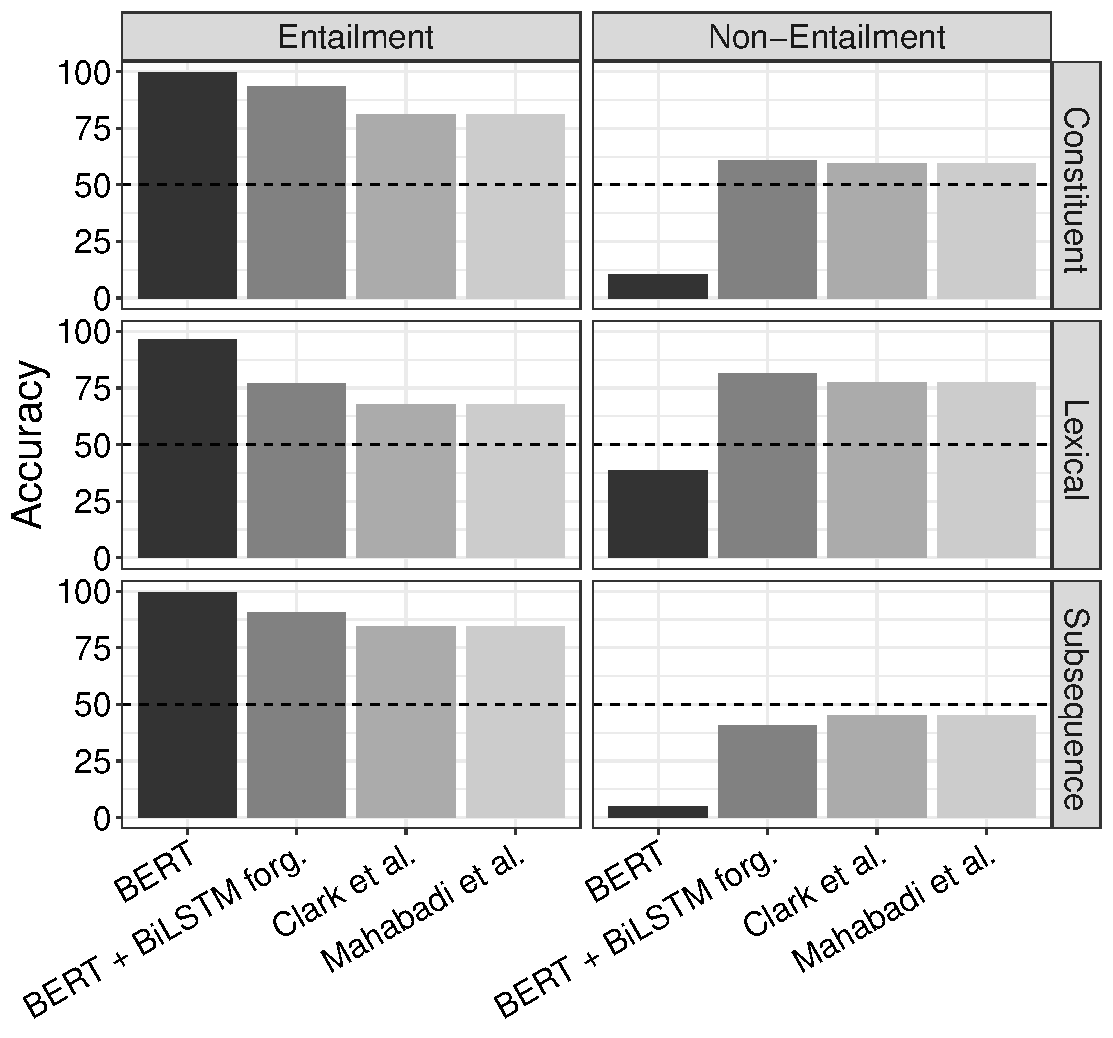
\includegraphics[scale=0.42]{figures/heuristic_plot.pdf}
\caption{Performance of our best model, BERT fine-tuned on the BiLSTM forgettables \flstm, versus the baselines for ``entailment'' and ``non-entailment'' categories for each heuristic the HANS test set was designed to capture. Our approach seems to better retain performance for entailment while still increasing accuracy over the baselines for non-entailment, albeit to a smaller extent.}
\label{fig:fine_eval_baselines}
\end{figure}

\subsection{A closer look into models predictions on HANS}
Here we look into the confidence of entailment in HANS
and MNLI evaluation sets.

First, we show that BERT trained on all MNLI examples is able
to discriminate HANS entailments from non-entailments but with
a much higher threshold than 0.5. 
Finetuning on forgettables calibrates classification
threshold on HANS and makes 0.5 as the optimum value of threshold.

\begin{figure}
    \centering
    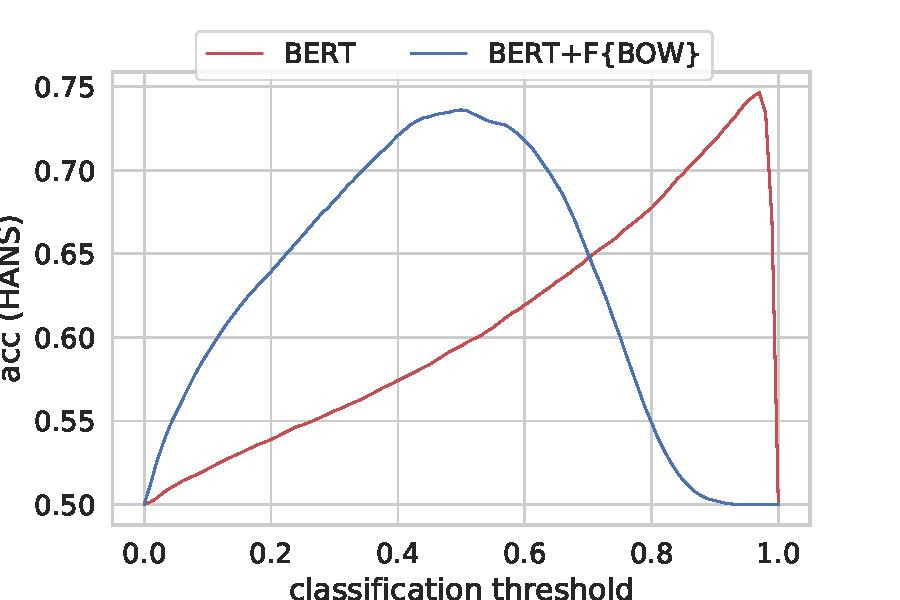
\includegraphics[width=0.4\textwidth]{figures/threshold_hans.pdf}
    \caption{Classification threshold vs HANS accuracy}
    \label{fig:threshold_hans}
\end{figure}

Second, we show the histogram of the models' entailment confidence 
in HANS examples.

\begin{figure}
    \centering
    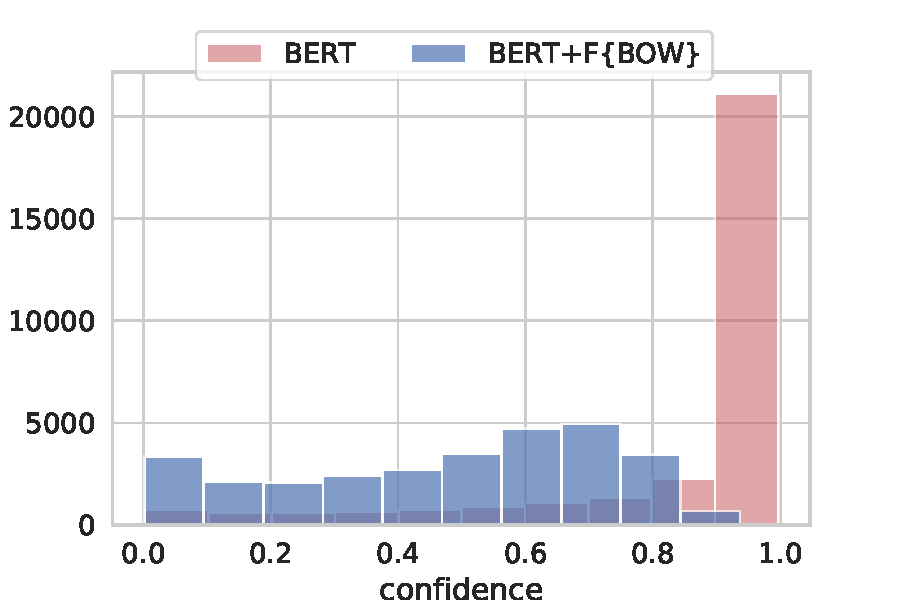
\includegraphics[width=0.5\textwidth]{figures/confidence_hans_hist.pdf}
    \caption{Confidence Histogram on HANS.}
    \label{fig:confidence_hans}
\end{figure}
